%%%%%%%%%%%%%%%%%%%%%%%%%%%%%%%%%%%%%%%%%%%%%%%%%%%%%%%%%%%%%%%%%%%%%%%%%%%%%%%%%%
\begin{frame}[fragile]\frametitle{}
\begin{center}
{\Large Agents using SmolAgents}
\end{center}
\end{frame}

%%%%%%%%%%%%%%%%%%%%%%%%%%%%%%%%%%%%%%%%%%%%%%%%%%%%%%%%%%%
\begin{frame}[fragile]\frametitle{SmolAgents at a Glance: Many Agents, One Framework}
      \begin{itemize}
	\item Unified framework with multiple agent types and capabilities
	\item Vision + Browser Agents interpret visual data and navigate web
	\item Code Agents write Python code as actions for complex tasks
	\item Tool-Calling Agents use structured JSON calls or text instructions
	\item Multi-Agents orchestrate multiple agents in hierarchical workflows
	\item Retrieval Agents use RAG to pull information from knowledge bases
	\item Built-in tools: web search, Python interpreter, speech-to-text
	\item Customizable tool functions enable real-world agent actions
	  \end{itemize}
\end{frame}

%%%%%%%%%%%%%%%%%%%%%%%%%%%%%%%%%%%%%%%%%%%%%%%%%%%%%%%%%%%
\begin{frame}[fragile]\frametitle{Code vs JSON: SmolAgent's Code-First Philosophy}
      \begin{itemize}
	\item Agents call tools by writing code instead of filling JSON schemas
	\item Traditional frameworks use structured JSON: \{"action": "Search", "input": "tutorials"\}
	\item Code-first offers full Python logic: loops, branches, complex operations
	\item Multiple tool calls in one go reduces iteration cycles by ~30\%
	\item Fewer reasoning steps while achieving better results than JSON approaches
	\item Code provides visible thought process, simplifying debugging
	\item JSON option available via ToolCallingAgent for simpler tasks
	\item Safety handled through secure interpreters and sandboxes
	  \end{itemize}
\end{frame}

%%%%%%%%%%%%%%%%%%%%%%%%%%%%%%%%%%%%%%%%%%%%%%%%%%%%%%%%%%%
\begin{frame}[fragile]\frametitle{Inside the CodeAgent Loop: How Does It Work?}


      \begin{itemize}
		\item Agent receives task and initializes system prompt with available tools
		\item LLM generates next action as executable Python code snippet
		\item Generated code runs and executes tool calls, returning results
		\item Results captured and appended to agent's conversation history
		\item Agent uses updated context to decide next action iteratively
		\item Agent calls final\_answer(answer\_text) when task complete
		\item Memory ensures continuity, prevents repetition and contradictions
		\item Error handling allows reconsideration when code bugs or failures occur
		\item Follows ReAct paradigm (Reason + Act) with code-based actions
	  \end{itemize}


\end{frame}

%%%%%%%%%%%%%%%%%%%%%%%%%%%%%%%%%%%%%%%%%%%%%%%%%%%%%%%%%%%
\begin{frame}[fragile]\frametitle{Inside the CodeAgent Loop: How Does It Work?}


		\begin{center}
		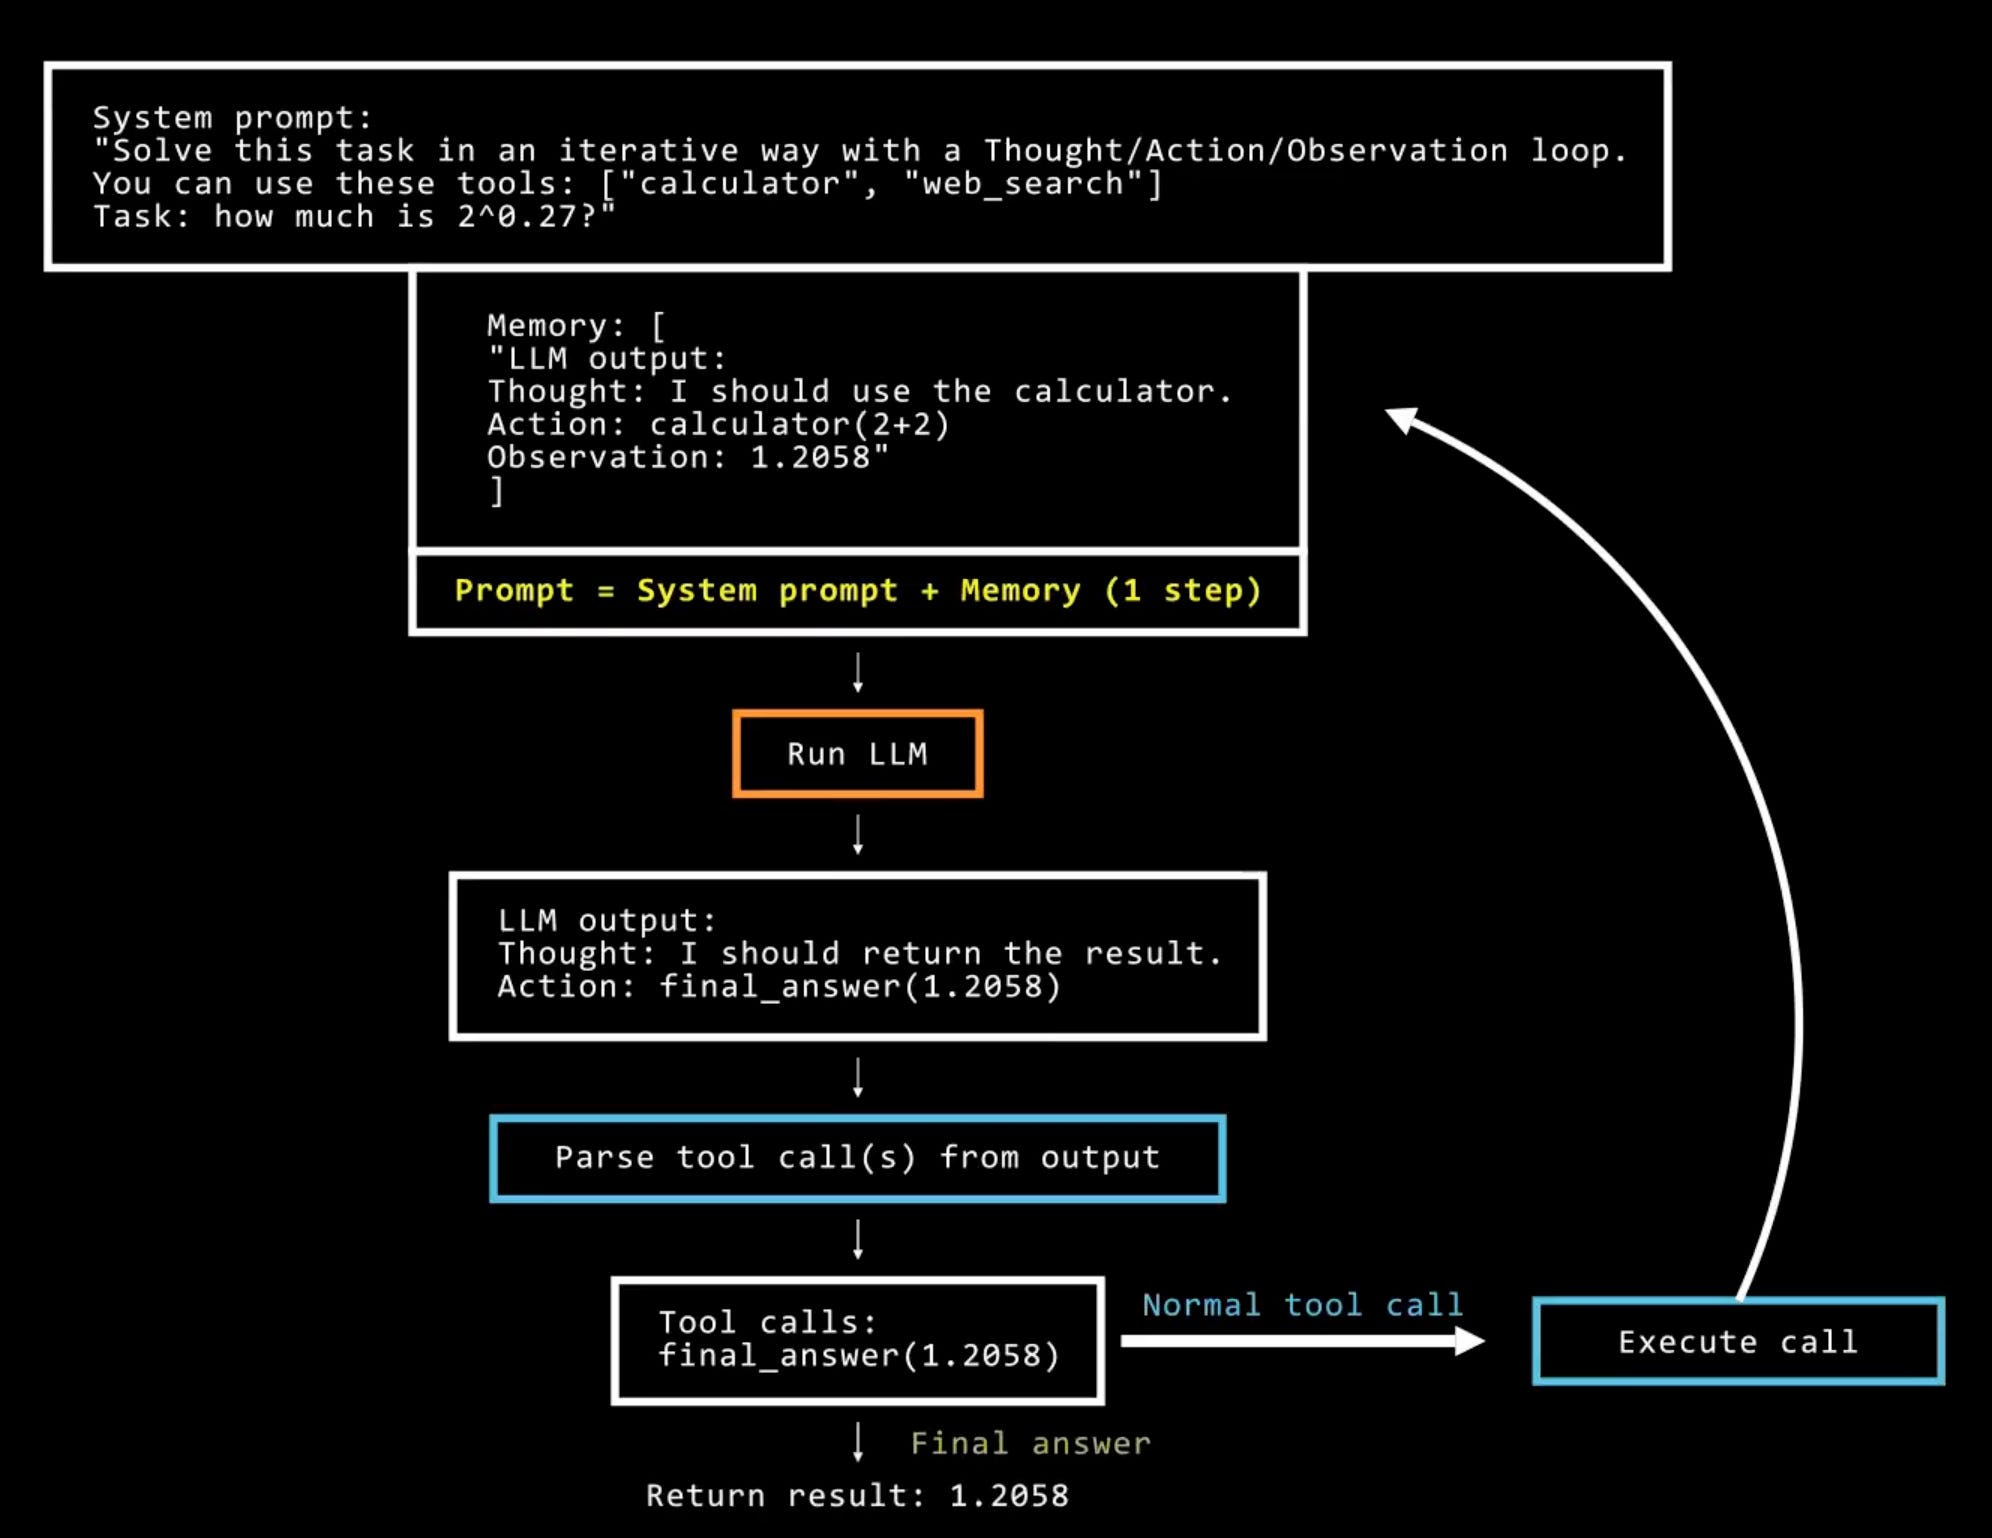
\includegraphics[width=0.8\linewidth,keepaspectratio]{aiagents56}
		
		{\tiny (Ref: Vizuara AI Agents Bootcamp Day 6)}

		\end{center}	

  

\end{frame}

%%%%%%%%%%%%%%%%%%%%%%%%%%%%%%%%%%%%%%%%%%%%%%%%%%%%%%%%%%%
\begin{frame}[fragile]\frametitle{ToolCallingAgent vs CodeAgent: A Quick Comparison}
      \begin{itemize}
	\item Both use same underlying multi-step ReAct logic
	\item ToolCallingAgent uses structured JSON calls for predictable interactions
	\item CodeAgent enables complex logic and multi-step operations in single thought
	\item ToolCallingAgent better for quick prototyping and safe environments
	\item CodeAgent superior for complex sequences requiring full programming
	\item Both accomplish complex tasks but serve different use cases
	\item Framework allows choosing between styles based on specific needs
	\item Code approach requires safety considerations but offers greater capability
	  \end{itemize}
\end{frame}

%%%%%%%%%%%%%%%%%%%%%%%%%%%%%%%%%%%%%%%%%%%%%%%%%%%%%%%%%%%
\begin{frame}[fragile]\frametitle{ToolCallingAgent vs CodeAgent}
	
	\begin{center}
	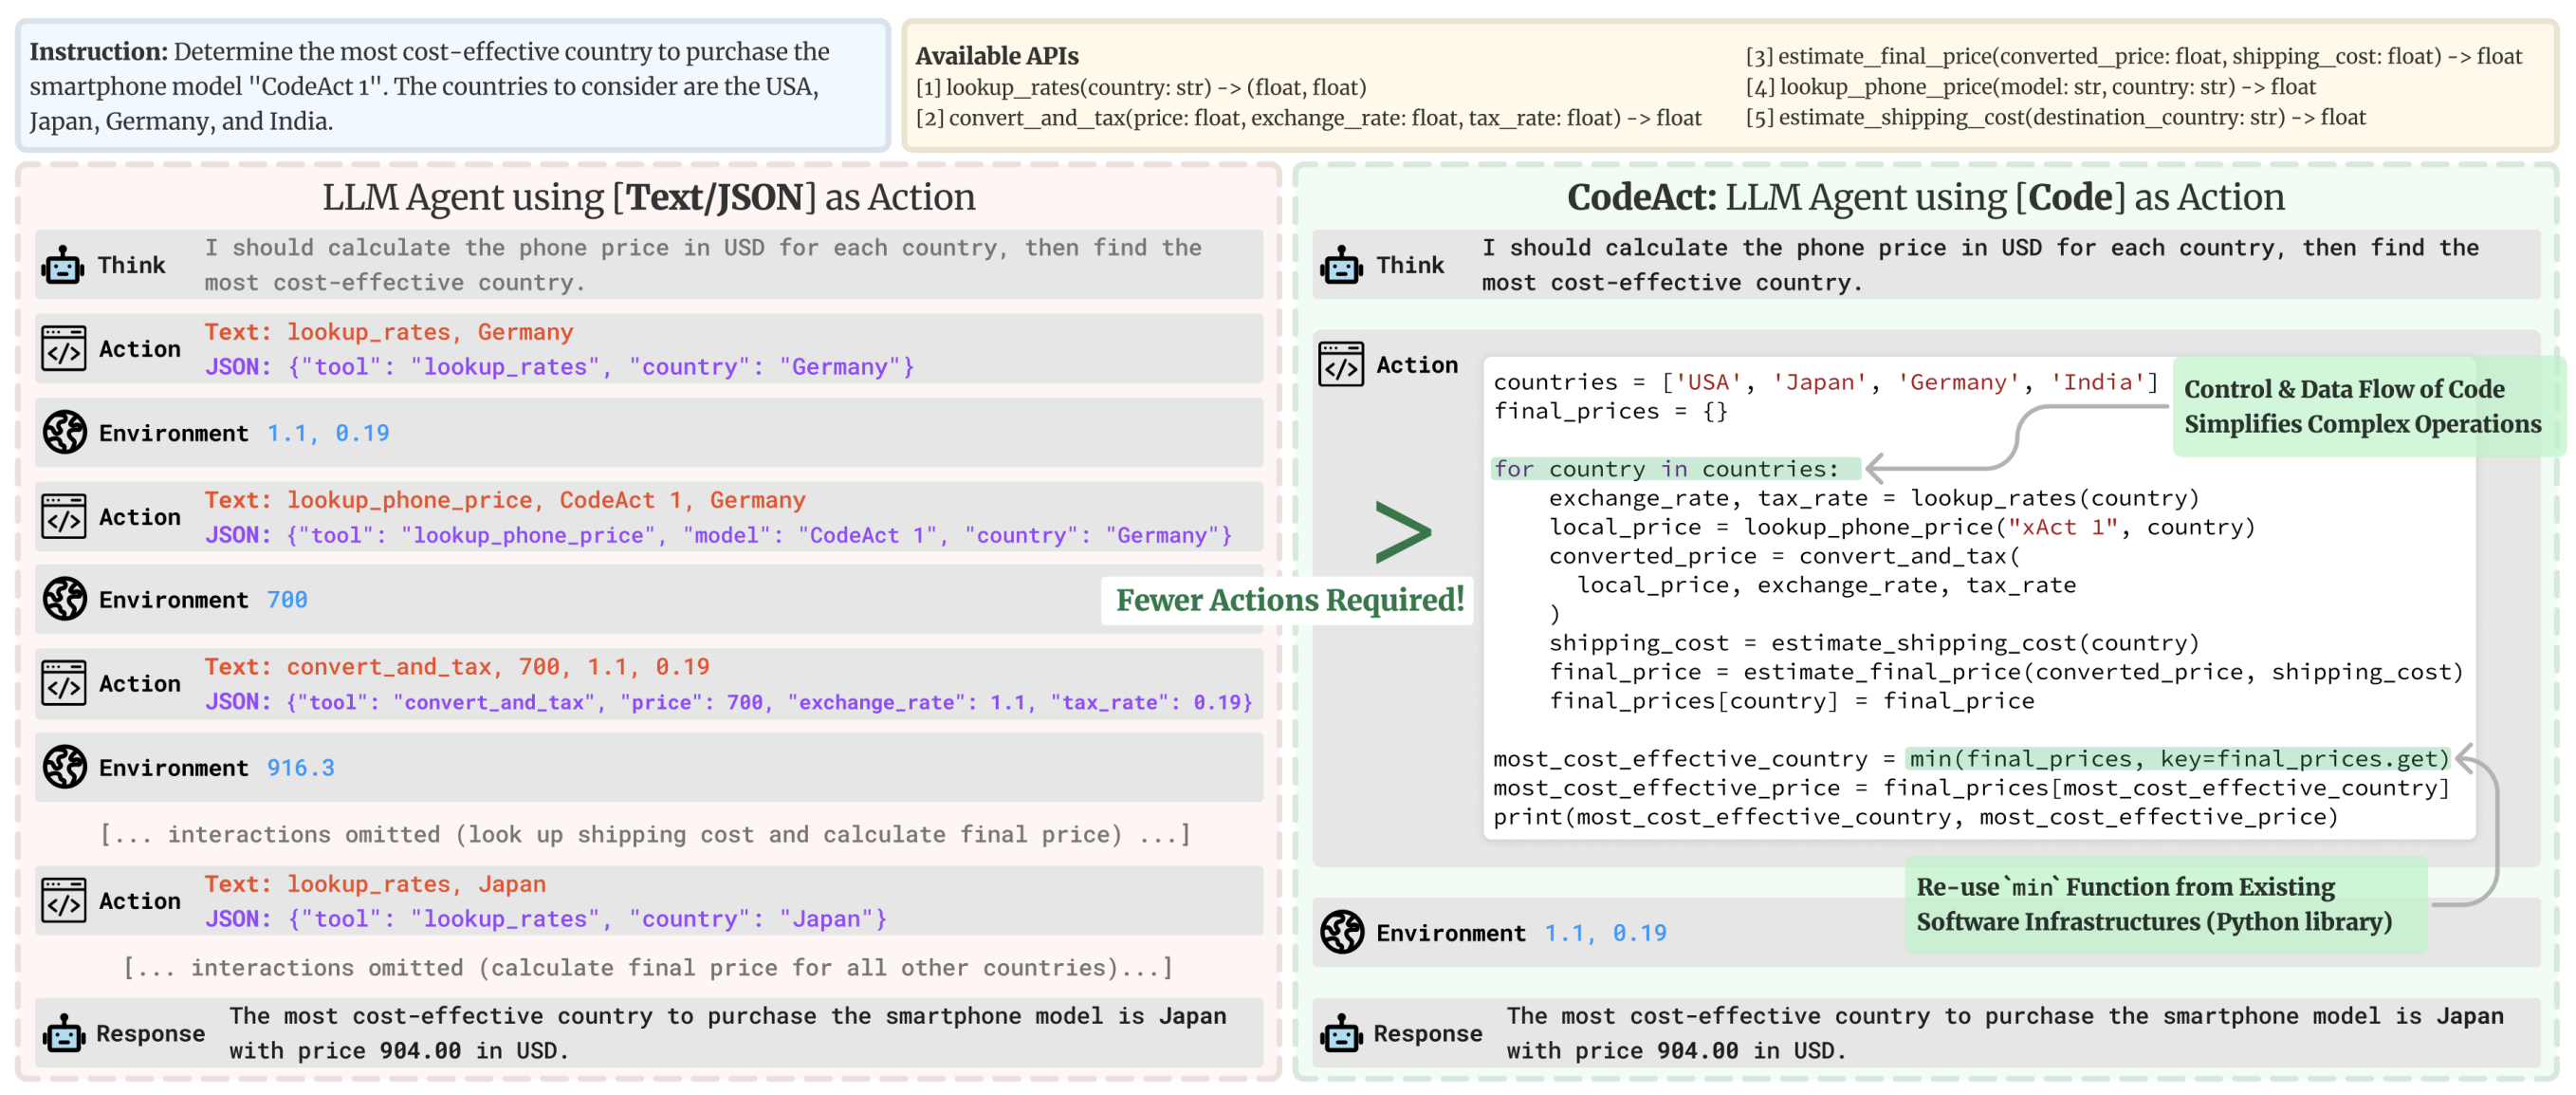
\includegraphics[width=\linewidth,keepaspectratio]{aiagents47}
	
	{\tiny (Ref: Writing actions as code snippets or JSON blobs - Hugging Face)}
	\end{center}
	
\end{frame}

%%%%%%%%%%%%%%%%%%%%%%%%%%%%%%%%%%%%%%%%%%%%%%%%%%%%%%%%%%%
\begin{frame}[fragile]\frametitle{Vision Agents}
      \begin{itemize}
	\item Vision Agents accept and process image inputs
	\item Analyze visual data: charts, screenshots, webpage images
	\item Enable UI automation by interpreting visual elements
	\item Support vision models for image-based tasks
	\item Control web browsers by interpreting screenshots and page elements
	\item Combine visual perception with other tools in agent toolbox
	\item Enable multimodal AI interactions beyond text-only processing
	  \end{itemize}
\end{frame}

%%%%%%%%%%%%%%%%%%%%%%%%%%%%%%%%%%%%%%%%%%%%%%%%%%%%%%%%%%%
\begin{frame}[fragile]\frametitle{LangFuse: Observability for LLM Agents}

	  
\begin{columns}
    \begin{column}[T]{0.6\linewidth}
      \begin{itemize}
	\item Observability platform tailored for LLM agents
	\item Enables tracking, visualizing, and debugging agent outputs
	\item Logs agent actions, tool calls, and reasoning steps
	\item Provides insights into agent behavior and performance bottlenecks
	\item Helps understand logic flow and identify improvement areas
	\item Essential companion for building robust, transparent AI agents
	\item Facilitates effortless monitoring and debugging of agent workflows
	  \end{itemize}
    \end{column}
    \begin{column}[T]{0.4\linewidth}
		\begin{center}
		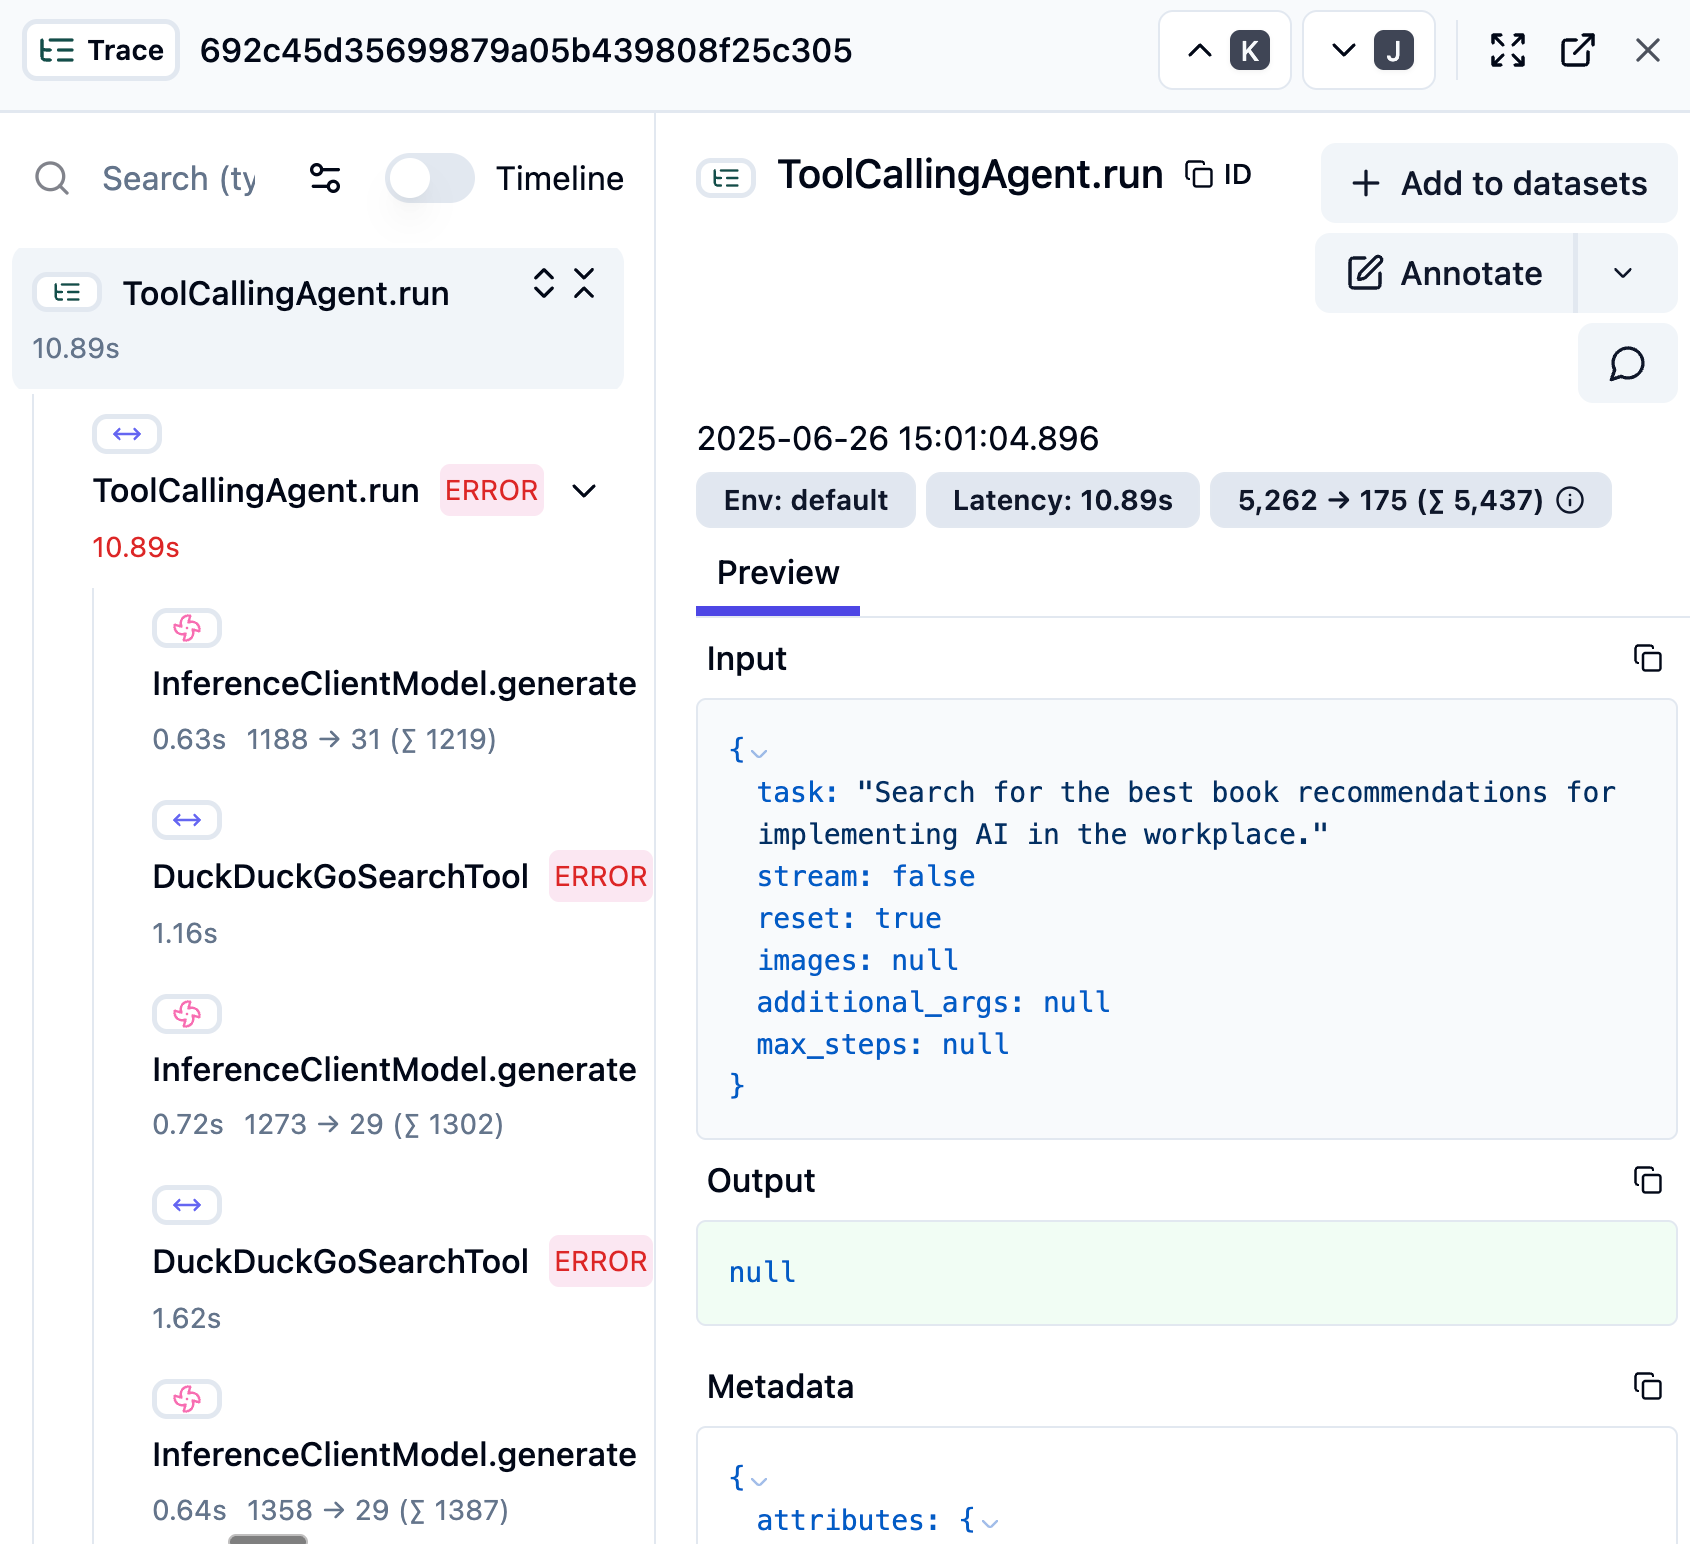
\includegraphics[width=0.8\linewidth,keepaspectratio]{aiagents57}
		
		{\tiny (Ref: Vizuara AI Agents Bootcamp Day 6)}

		\end{center}	
    \end{column}
  \end{columns}	  
\end{frame}

%%%%%%%%%%%%%%%%%%%%%%%%%%%%%%%%%%%%%%%%%%%%%%%%%%%%%%%%%%%
\begin{frame}[fragile]\frametitle{Basic Agent Setup: CodeAgent}
\begin{columns}
\begin{column}{0.5\textwidth}
      \begin{itemize}
	\item Minimal agent requires model and tools arguments
	\item HfApiModel leverages Hugging Face Inference API
	\item CodeAgent executes Python code snippets at each step
	\item add\_base\_tools=True includes default toolbox
	\item Built-in safety with predefined safe functions only
	\item Execution stops on illegal operations or Python errors
	  \end{itemize}
\end{column}
\begin{column}{0.5\textwidth}
\begin{lstlisting}[language=Python, basicstyle=\tiny]
from smolagents import CodeAgent, HfApiModel

# Initialize model using HF API
model = HfApiModel(
    model_id="meta-llama/Llama-3.3-70B-Instruct"
)

# Create agent with default tools
agent = CodeAgent(
    tools=[], 
    model=model, 
    add_base_tools=True
)

# Run agent with task
result = agent.run(
    "Calculate the 118th Fibonacci number"
)
\end{lstlisting}
\end{column}
\end{columns}
\end{frame}

%%%%%%%%%%%%%%%%%%%%%%%%%%%%%%%%%%%%%%%%%%%%%%%%%%%%%%%%%%%
\begin{frame}[fragile]\frametitle{Custom Tool Creation: @tool Decorator}
\begin{columns}
\begin{column}{0.5\textwidth}
      \begin{itemize}
	\item @tool decorator converts functions into agent tools
	\item Requires clear name, type hints, and description
	\item Args section describes each parameter for LLM
	\item Tool description baked into agent's system prompt
	\item Same format as apply\_chat\_template tool schemas
	  \end{itemize}
\end{column}
\begin{column}{0.5\textwidth}
\begin{lstlisting}[language=Python, basicstyle=\tiny]
from smolagents import tool, CodeAgent, HfApiModel
from huggingface_hub import list_models

@tool
def model_download_tool(task: str) -> str:
    """
    Returns most downloaded model for given task.
    
    Args:
        task: Task for download count.
    """
    most_downloaded_model = next(iter(
        list_models(filter=task, sort="downloads", 
                   direction=-1)
    ))
    return most_downloaded_model.id

# Use custom tool
agent = CodeAgent(
    tools=[model_download_tool], 
    model=HfApiModel()
)
result = agent.run(
    "Most downloaded text-to-video model?"
)
\end{lstlisting}
\end{column}
\end{columns}
\end{frame}

%%%%%%%%%%%%%%%%%%%%%%%%%%%%%%%%%%%%%%%%%%%%%%%%%%%%%%%%%%%
\begin{frame}[fragile]\frametitle{Multi-Agent Systems: ManagedAgent}
\begin{columns}
\begin{column}{0.5\textwidth}
      \begin{itemize}
	\item Hierarchical multi-agent systems for better specialization
	\item ManagedAgent encapsulates agents as tools for manager
	\item Requires agent, name, and description arguments
	\item Separate tool sets and memories for efficient specialization
	\item Manager agent coordinates specialized sub-agents
	\item Better performance on complex benchmarks
	  \end{itemize}
\end{column}
\begin{column}{0.5\textwidth}
\begin{lstlisting}[language=Python, basicstyle=\tiny]
from smolagents import (CodeAgent, HfApiModel, 
                       DuckDuckGoSearchTool, ManagedAgent)

model = HfApiModel()

# Create specialized web search agent
web_agent = CodeAgent(
    tools=[DuckDuckGoSearchTool()], 
    model=model
)

# Wrap as managed agent
managed_web_agent = ManagedAgent(
    agent=web_agent,
    name="web_search",
    description="Runs web searches. "
               "Give query as argument."
)

# Create manager agent
manager_agent = CodeAgent(
    tools=[], 
    model=model, 
    managed_agents=[managed_web_agent]
)

result = manager_agent.run(
    "Who is the CEO of Hugging Face?"
)
\end{lstlisting}
\end{column}
\end{columns}
\end{frame}

%%%%%%%%%%%%%%%%%%%%%%%%%%%%%%%%%%%%%%%%%%%%%%%%%%%%%%%%%%%
\begin{frame}[fragile]\frametitle{ToolCallingAgent vs CodeAgent Examples}
\begin{columns}
\begin{column}{0.5\textwidth}
      \begin{itemize}
	\item ToolCallingAgent uses JSON-like action blobs
	\item CodeAgent executes Python code for actions
	\item Same initialization pattern, different execution styles
	\item ToolCallingAgent safer, CodeAgent more flexible
	\item additional\_authorized\_imports for CodeAgent only
	  \end{itemize}
\end{column}
\begin{column}{0.5\textwidth}
\begin{lstlisting}[language=Python, basicstyle=\tiny]
from smolagents import (CodeAgent, ToolCallingAgent, 
                       HfApiModel)

model = HfApiModel()

# ToolCallingAgent - JSON-style actions
tool_agent = ToolCallingAgent(
    tools=[], 
    model=model
)
result1 = tool_agent.run(
    "Get title of https://huggingface.co/blog"
)

# CodeAgent - Code execution with imports
code_agent = CodeAgent(
    tools=[], 
    model=model, 
    additional_authorized_imports=[
        'requests', 'bs4'
    ]
)
result2 = code_agent.run(
    "Get title of https://huggingface.co/blog"
)
\end{lstlisting}
\end{column}
\end{columns}
\end{frame}

%%%%%%%%%%%%%%%%%%%%%%%%%%%%%%%%%%%%%%%%%%%%%%%%%%%%%%%%%%%
\begin{frame}[fragile]\frametitle{Agent Inspection and Gradio UI}
\begin{columns}
\begin{column}{0.5\textwidth}
      \begin{itemize}
	\item agent.logs stores fine-grained execution logs
	\item write\_inner\_memory\_from\_logs() creates LLM-viewable memory
	\item GradioUI provides interactive chat interface
	\item reset=False maintains conversation memory
	\item Visualize agent thoughts and execution process
	  \end{itemize}
\end{column}
\begin{column}{0.5\textwidth}
\begin{lstlisting}[language=Python, basicstyle=\tiny]
from smolagents import (CodeAgent, HfApiModel, 
                       GradioUI, load_tool)

# Load tool from Hub
image_tool = load_tool("m-ric/text-to-image")

# Initialize agent
model = HfApiModel()
agent = CodeAgent(
    tools=[image_tool], 
    model=model
)

# Launch interactive interface
GradioUI(agent).launch()

# Inspect agent after run
print(agent.logs)  # Fine-grained logs
agent.write_inner_memory_from_logs()  
# LLM-viewable memory

# Continue conversation
agent.run("Follow up question", reset=False)
\end{lstlisting}
\end{column}
\end{columns}
\end{frame}

%%%%%%%%%%%%%%%%%%%%%%%%%%%%%%%%%%%%%%%%%%%%%%%%%%%%%%%%%%%%%%%%%%%%%%%%%%%%%%%%%%
\begin{frame}[fragile]\frametitle{}
\begin{center}
{\Large Multi-Agents using SmolAgents}
\end{center}
\end{frame}

%%%%%%%%%%%%%%%%%%%%%%%%%%%%%%%%%%%%%%%%%%%%%%%%%%%%%%%%%%%
\begin{frame}[fragile]\frametitle{Why Multi-Agent Systems? From Solo to Teamwork}

      \begin{itemize}
		\item Single agents handling everything aren't always ideal for complex tasks
		\item Multi-agent systems enable specialized agents working together toward common goals
		\item Each agent focuses on specific sub-tasks or roles with clear responsibilities
		\item Agents communicate and coordinate like an AI team
		\item Brings teamwork concepts to AI agents for better performance
		\item More robust and performant than monolithic single agents
	  \end{itemize}

\end{frame}

%%%%%%%%%%%%%%%%%%%%%%%%%%%%%%%%%%%%%%%%%%%%%%%%%%%%%%%%%%%
\begin{frame}[fragile]\frametitle{Key Advantages of Multi-Agent Systems}

      \begin{itemize}
		\item \textbf{Divide and Conquer:} Each agent has single responsibility, simplifying complex problems
		\item \textbf{Parallelism \& Speed:} Agents work in parallel or sequentially with less overhead
		\item \textbf{Improved Focus \& Memory:} Each agent maintains its own context, reducing prompt size
		\item \textbf{Fault Tolerance:} If one agent fails, others can catch issues or request retries
		\item \textbf{Specialization:} Different skill sets assigned to different agents (researcher, calculator, planner)
		\item \textbf{Cost Efficiency:} Smaller prompts per agent reduce latency and token costs
	  \end{itemize}

\end{frame}

%%%%%%%%%%%%%%%%%%%%%%%%%%%%%%%%%%%%%%%%%%%%%%%%%%%%%%%%%%%
\begin{frame}[fragile]\frametitle{Case Study: Harry Potter Trip Planner}
\begin{columns}
    \begin{column}[T]{0.6\linewidth}
      \begin{itemize}
		\item Complex task: Plan worldwide tour of Harry Potter filming locations
		\item Added twist: Include nearby cricket stadiums for sports fans
		\item Calculate travel times from Pune, India to each location
		\item Multiple sub-tasks requiring different specialized skills
		\item Perfect example of multi-step planning problem
		\item Demonstrates why single vs multi-agent approaches matter
	  \end{itemize}
    \end{column}
    \begin{column}[T]{0.4\linewidth}
		\begin{center}
		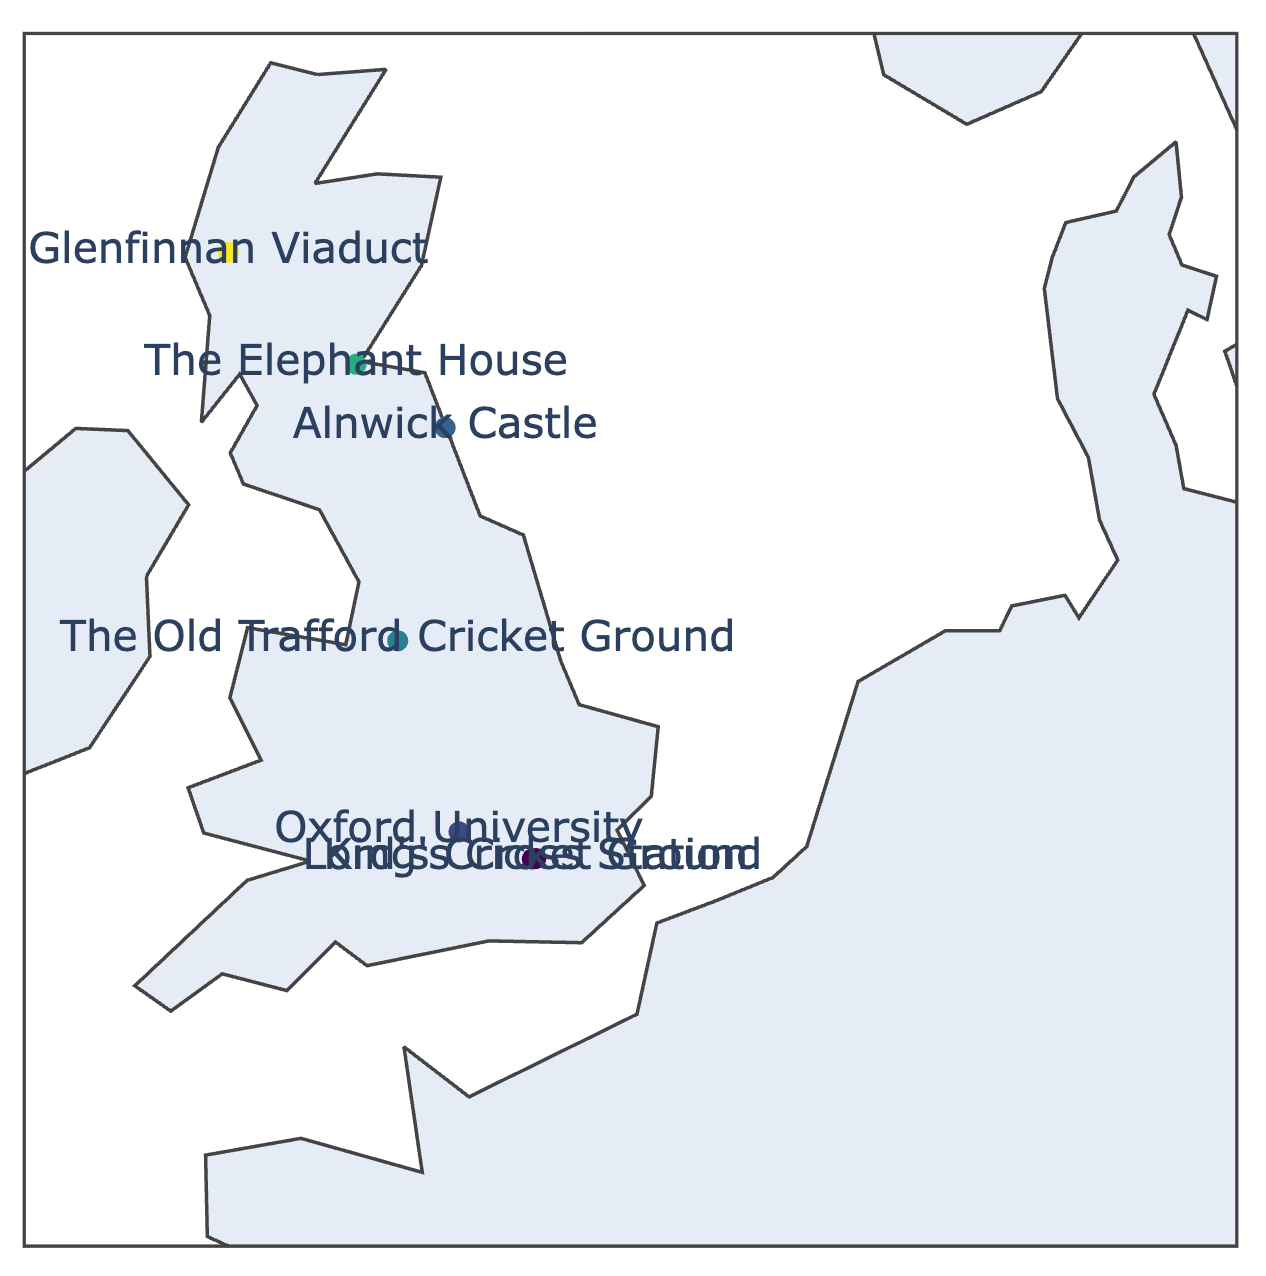
\includegraphics[width=0.8\linewidth,keepaspectratio]{aiagents51}
		
		{\tiny (Ref: Vizuara AI Agents Bootcamp Day 6)}
		\end{center}	
    \end{column}
  \end{columns}
\end{frame}

%%%%%%%%%%%%%%%%%%%%%%%%%%%%%%%%%%%%%%%%%%%%%%%%%%%%%%%%%%%
\begin{frame}[fragile]\frametitle{Single Agent Approach: Tools and Challenges}

      \begin{itemize}
		\item \textbf{Tools Used:} Web Search, Webpage Reader, Travel Time Calculator, Mapping Library
		\item Agent equipped with all necessary capabilities for end-to-end solution
		\item Successfully gathered data but hit significant limitations
		\item \textbf{Long Context Issue:} Prompt grew very large with all information
		\item \textbf{High Token Usage:} Expensive and slow due to context bloat
		\item \textbf{Complex Reasoning:} Juggling multiple tasks in one sequence increased errors
		\item Agent struggled to complete task within reasonable steps and token limits
	  \end{itemize}


\end{frame}

%%%%%%%%%%%%%%%%%%%%%%%%%%%%%%%%%%%%%%%%%%%%%%%%%%%%%%%%%%%
\begin{frame}[fragile]\frametitle{Single Agent Approach: Tools and Challenges}


		\begin{center}
		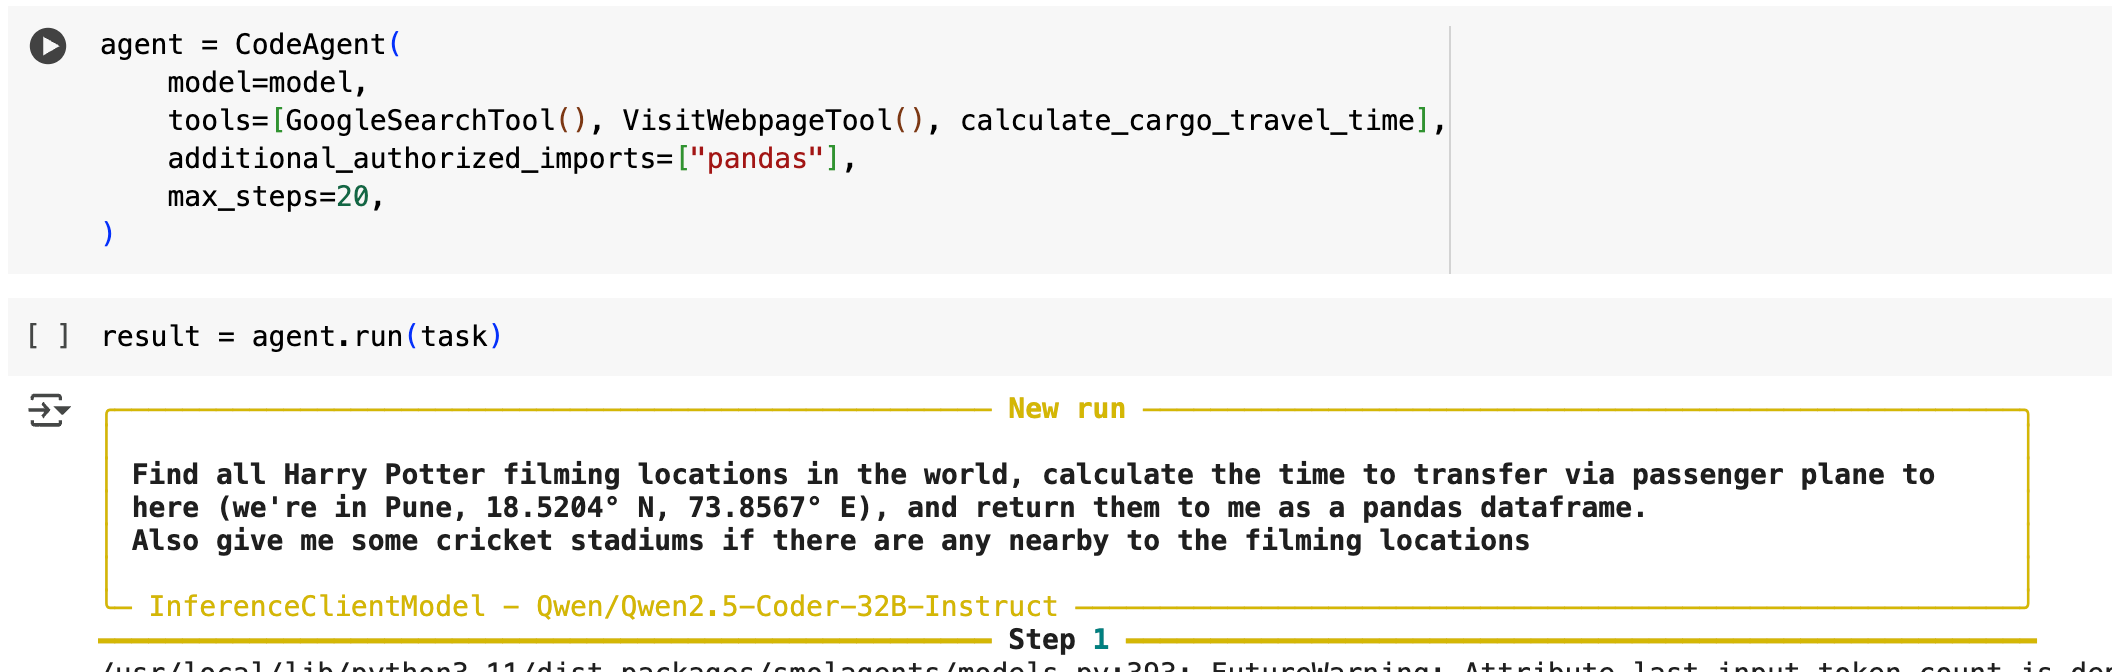
\includegraphics[width=0.8\linewidth,keepaspectratio]{aiagents48}
		
		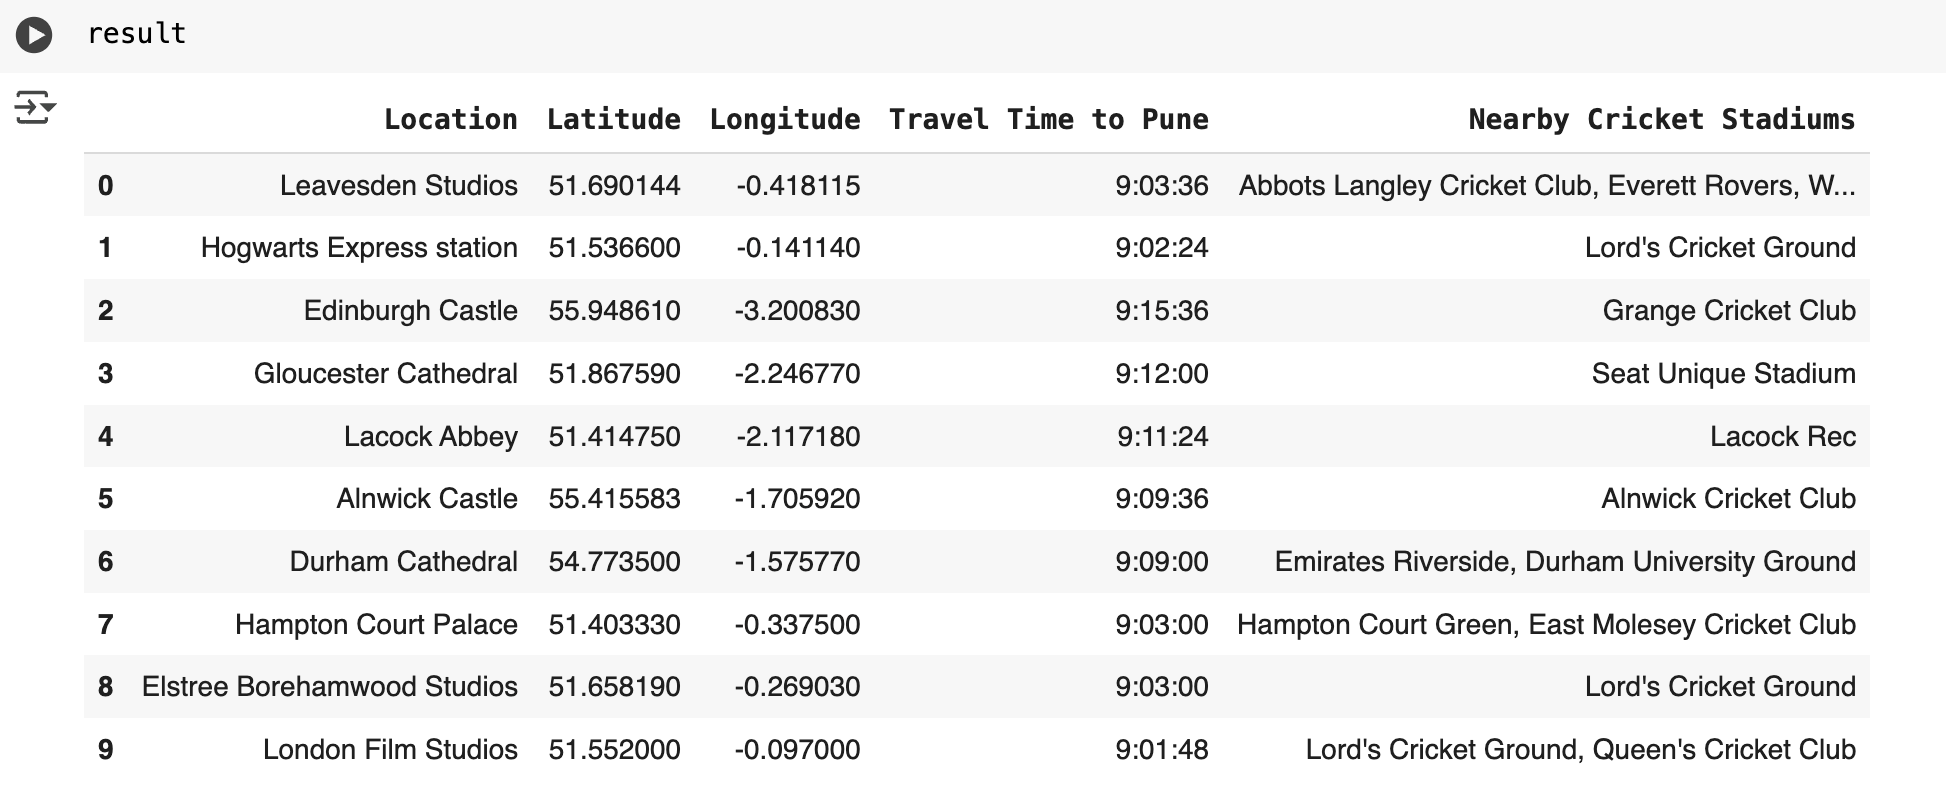
\includegraphics[width=0.8\linewidth,keepaspectratio]{aiagents49}
		
		{\tiny (Ref: Vizuara AI Agents Bootcamp Day 6)}
		\end{center}	

\end{frame}


%%%%%%%%%%%%%%%%%%%%%%%%%%%%%%%%%%%%%%%%%%%%%%%%%%%%%%%%%%%
\begin{frame}[fragile]\frametitle{Multi-Agent Solution: Division of Labor}

      \begin{itemize}
		\item \textbf{Browser Agent:} Specialist for web searching and reading tasks
		\item Responsible for finding filming locations and nearby stadiums
		\item Has access to internet tools and travel time calculator
		\item Returns structured data without worrying about final report
		\item \textbf{Manager Agent:} High-level project manager and finalizer
		\item Delegates work to browser agent and processes results
		\item Handles map generation and final output compilation
		\item Uses GPT-4 level model for analysis and output generation
	  \end{itemize}

\end{frame}

%%%%%%%%%%%%%%%%%%%%%%%%%%%%%%%%%%%%%%%%%%%%%%%%%%%%%%%%%%%
\begin{frame}[fragile]\frametitle{Multi-Agent Solution: Division of Labor}

		\begin{center}
		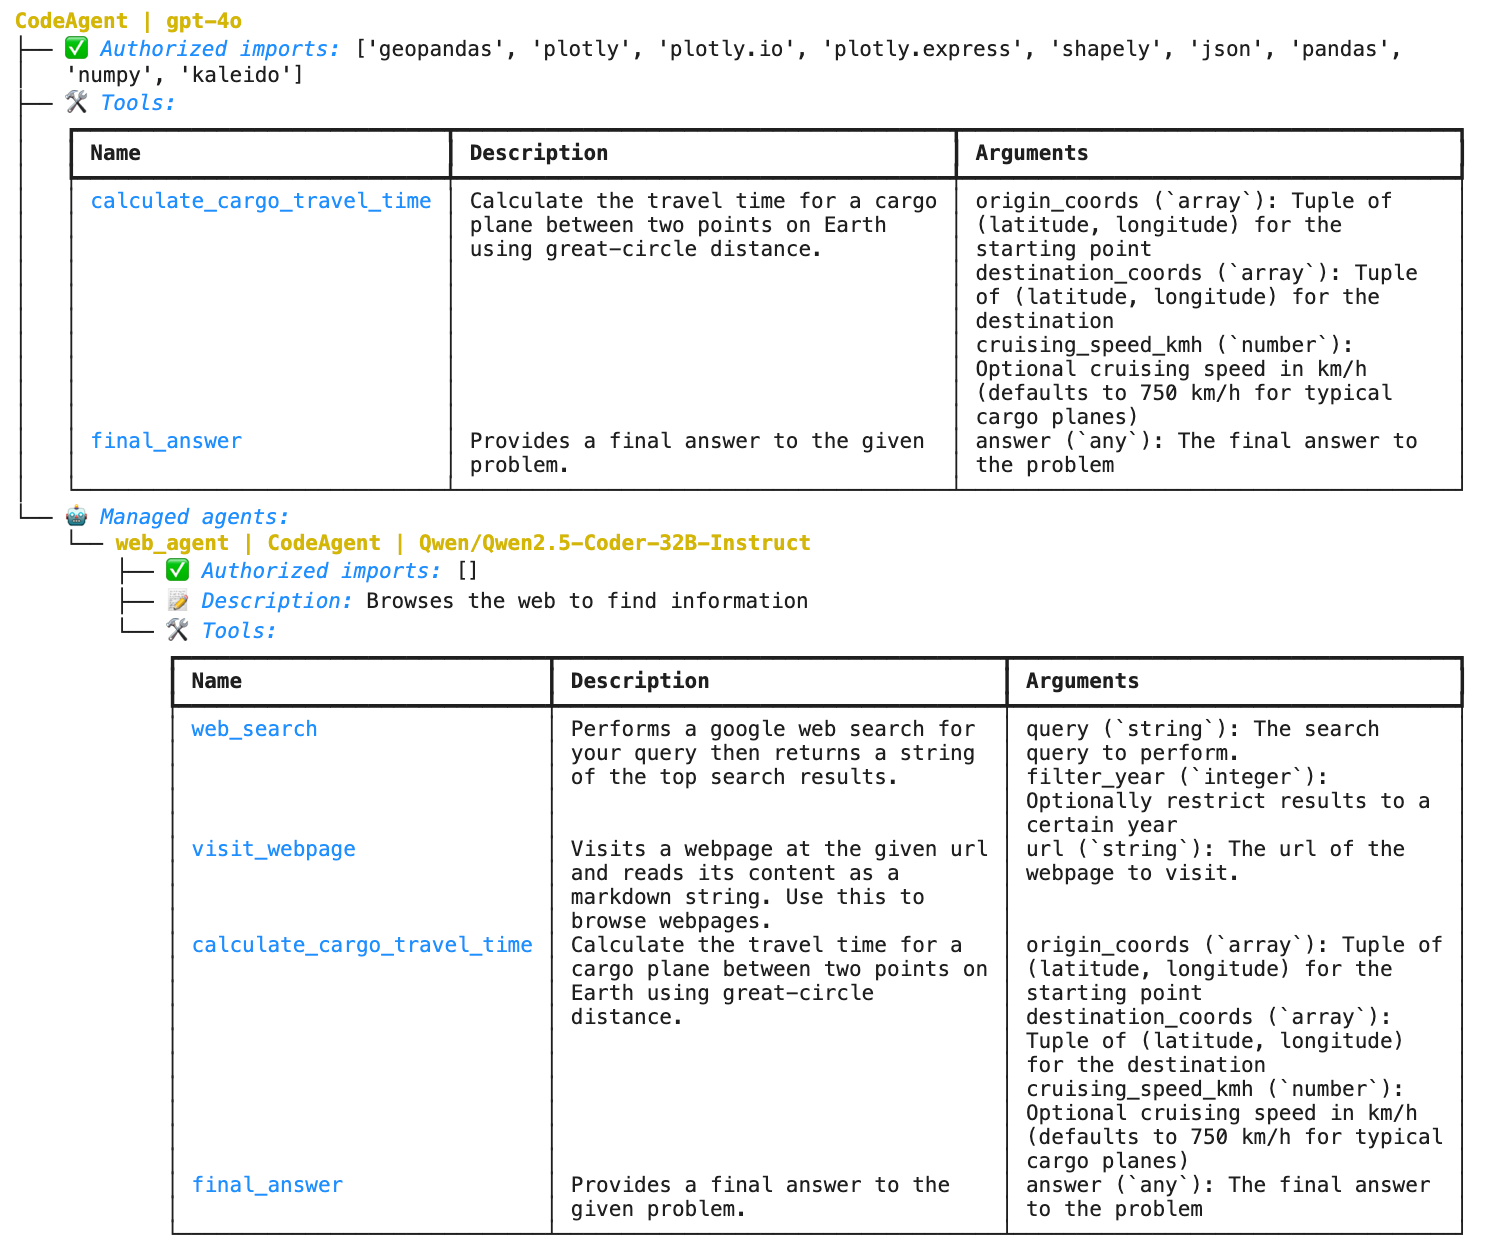
\includegraphics[width=0.7\linewidth,keepaspectratio]{aiagents50}
		
		{\tiny (Ref: Vizuara AI Agents Bootcamp Day 6)}
		\end{center}	

\end{frame}


%%%%%%%%%%%%%%%%%%%%%%%%%%%%%%%%%%%%%%%%%%%%%%%%%%%%%%%%%%%
\begin{frame}[fragile]\frametitle{Multi-Agent Benefits: Performance and Efficiency}
\begin{columns}
    \begin{column}[T]{0.6\linewidth}
      \begin{itemize}
		\item \textbf{Focused Context:} Each agent maintains smaller, specialized context
		\item Browser agent only keeps web search results and related info
		\item Manager agent starts with high-level view, doesn't need search details
		\item \textbf{Better Performance:} Each agent specialized and efficient at its task
		\item \textbf{Lower Token Usage:} Smaller prompts per agent reduce cost and latency
		\item Successful implementation of complex trip planner
		\item Generated comprehensive DataFrame and interactive map visualization
	  \end{itemize}
    \end{column}
    \begin{column}[T]{0.4\linewidth}
		\begin{center}
		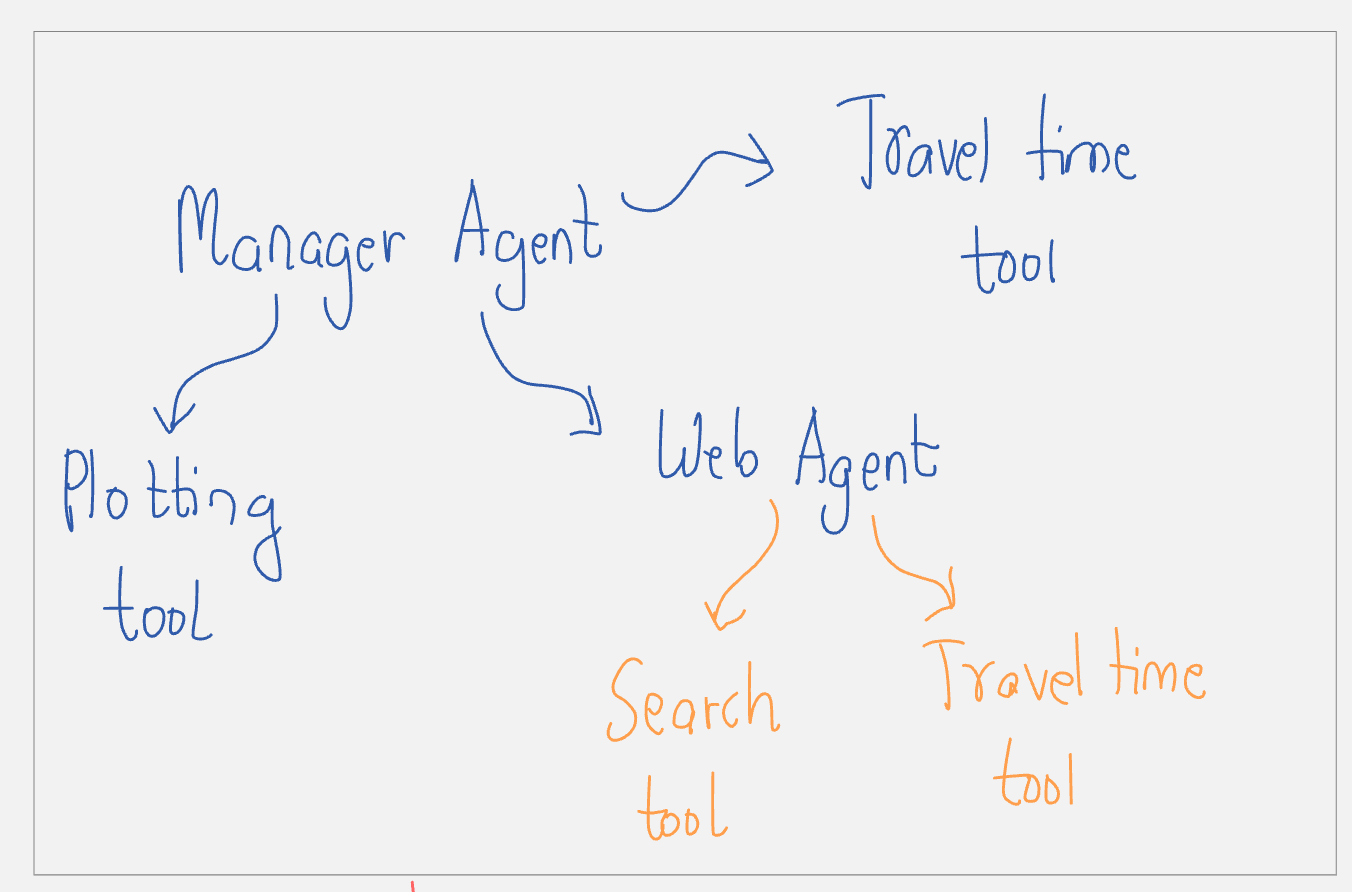
\includegraphics[width=0.8\linewidth,keepaspectratio]{aiagents52}
		
		{\tiny (Ref: Vizuara AI Agents Bootcamp Day 6)}
		\end{center}	
    \end{column}
  \end{columns}
\end{frame}

%%%%%%%%%%%%%%%%%%%%%%%%%%%%%%%%%%%%%%%%%%%%%%%%%%%%%%%%%%%
\begin{frame}[fragile]\frametitle{Langfuse: Tracing and Observability}

      \begin{itemize}
		\item Langfuse serves as control center and black box recorder for AI agents
		\item \textbf{Tracing:} Records sequence of operations and model calls in each task
		\item Logs agent messages, tool usage, intermediate results, and final outputs
		\item Provides timeline view showing steps in chronological order
		\item Essential for debugging when results are wrong or suboptimal
		\item Can pinpoint which step led agent astray in complex workflows
		\item Integration via environment variables and SDK with OpenTelemetry
	  \end{itemize}

\end{frame}

%%%%%%%%%%%%%%%%%%%%%%%%%%%%%%%%%%%%%%%%%%%%%%%%%%%%%%%%%%%
\begin{frame}[fragile]\frametitle{Langfuse: Tracing and Observability}


		\begin{center}
		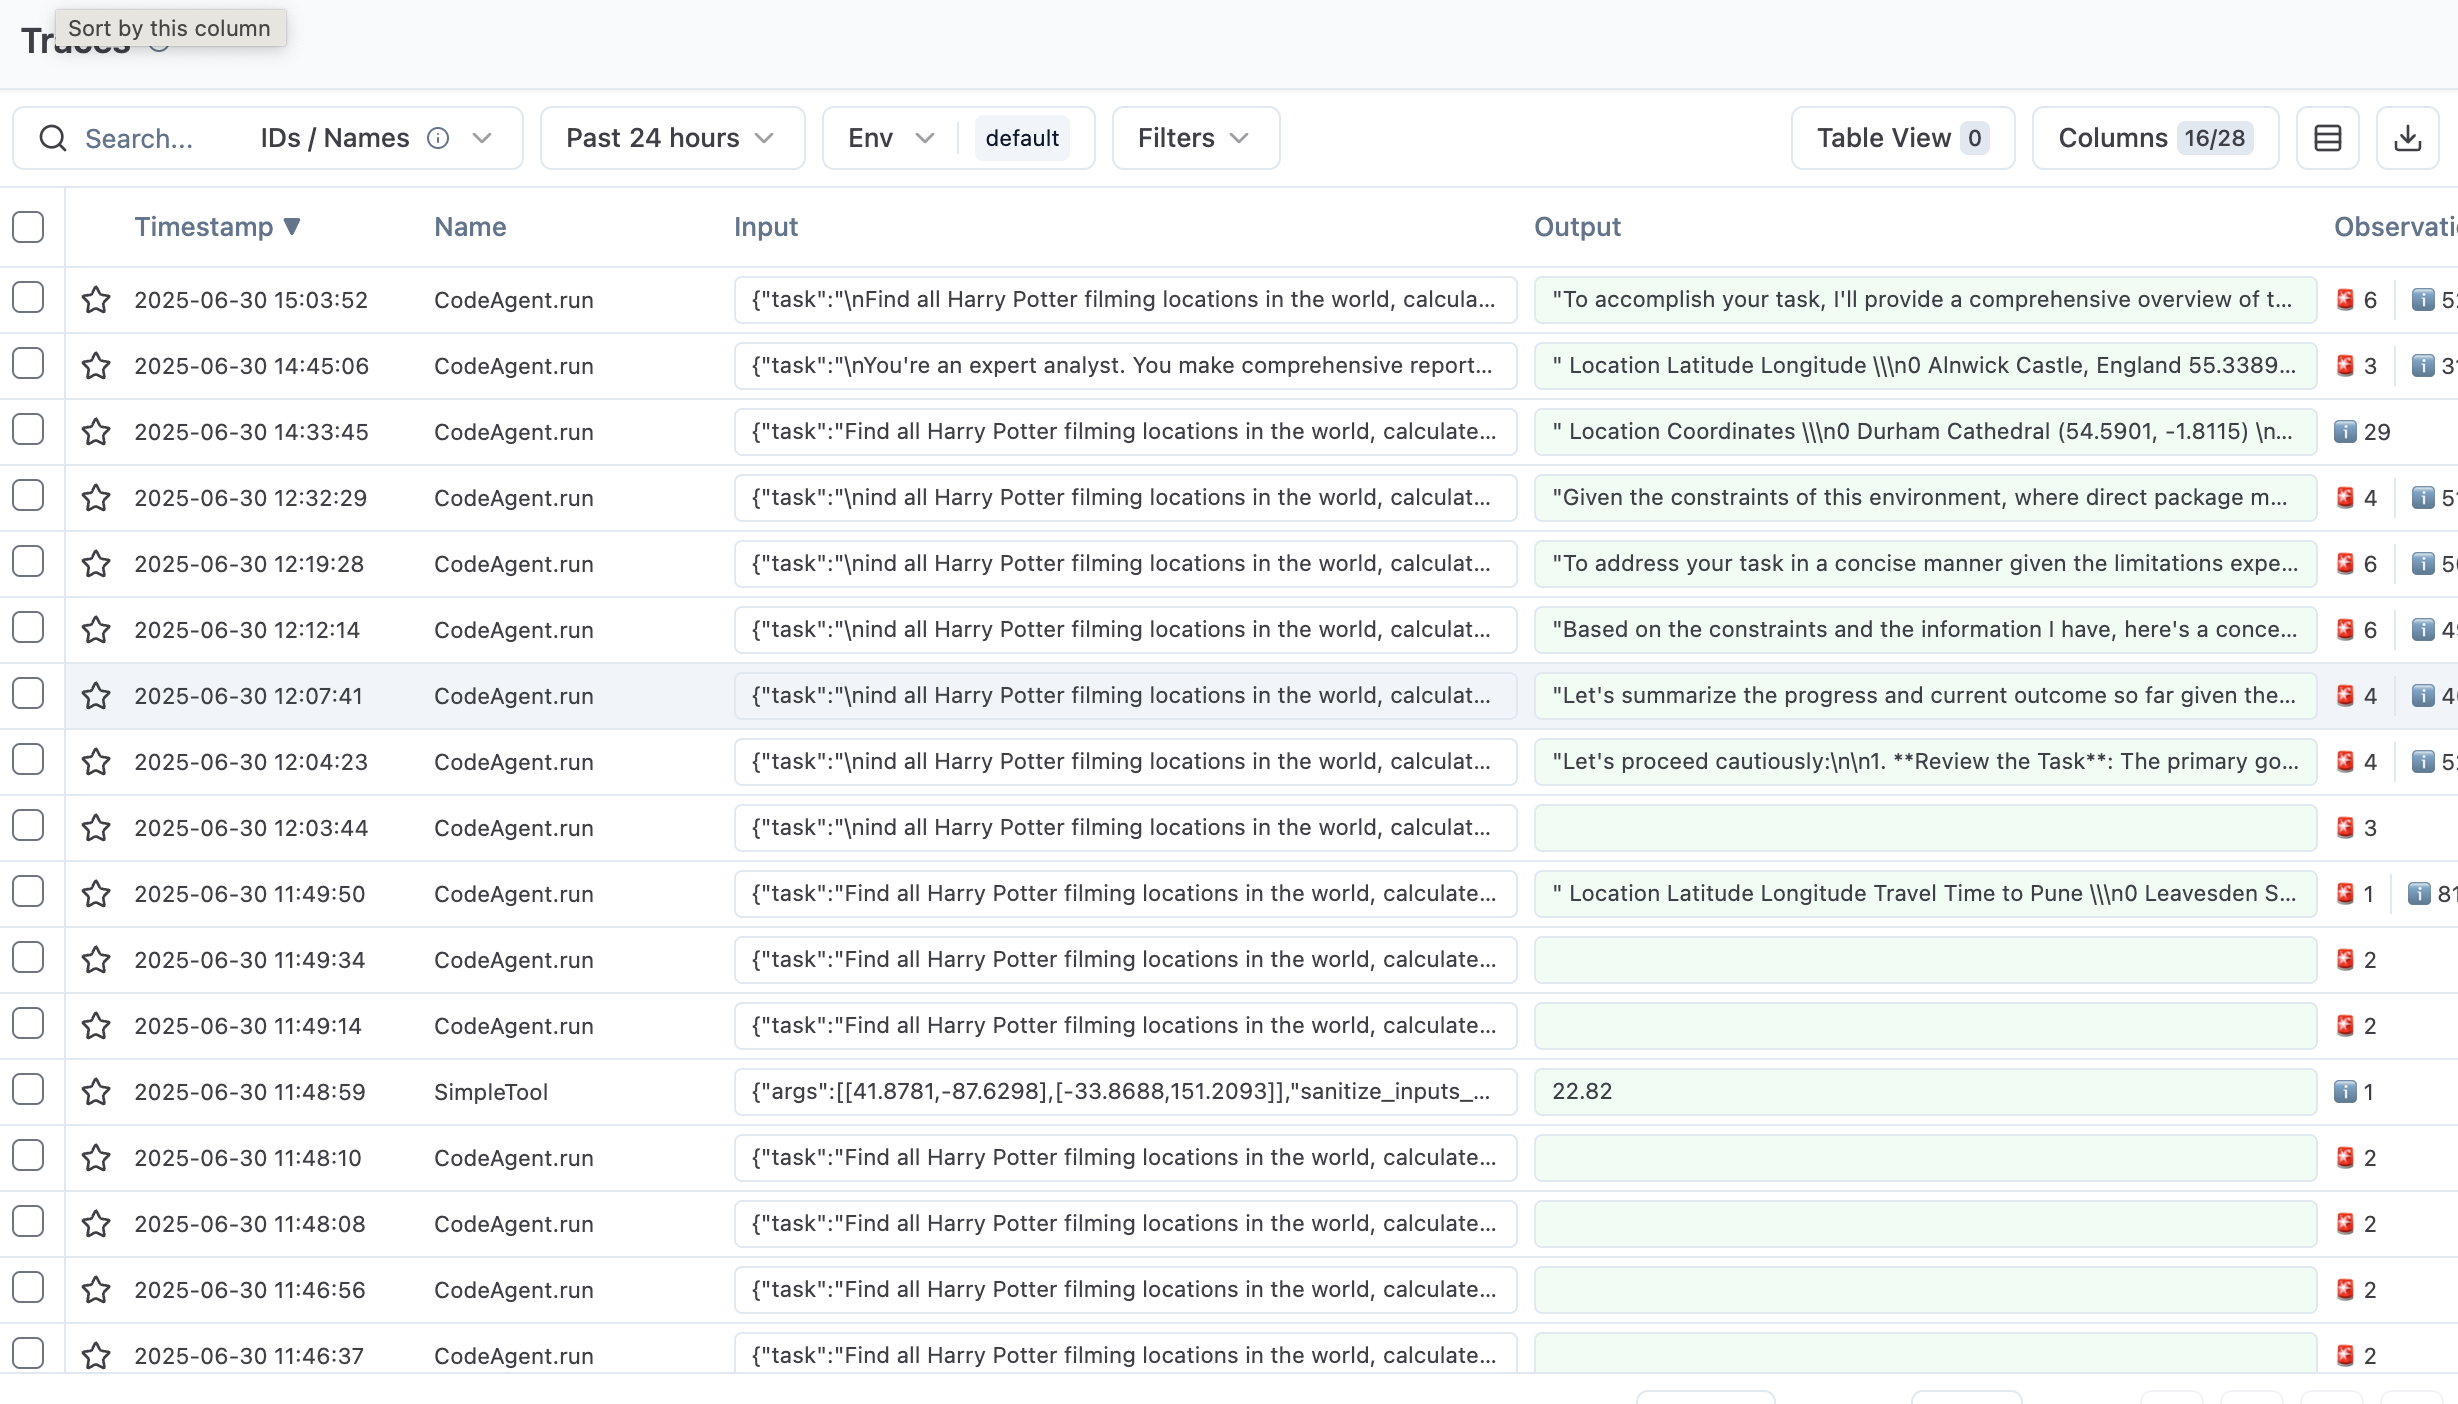
\includegraphics[width=\linewidth,keepaspectratio]{aiagents53}
		
		{\tiny (Ref: Vizuara AI Agents Bootcamp Day 6)}
		\end{center}	

\end{frame}


%%%%%%%%%%%%%%%%%%%%%%%%%%%%%%%%%%%%%%%%%%%%%%%%%%%%%%%%%%%
\begin{frame}[fragile]\frametitle{Building Evaluation Dashboard}
% \begin{columns}
    % \begin{column}[T]{0.6\linewidth}
      \begin{itemize}
		\item Langfuse enables building evaluation dashboard on top of traced data
		\item Define metrics to score each agent run and view aggregate analytics
		\item \textbf{Key Metrics:} Hallucinations, Trustworthiness, Relevance, Correctness
		\item \textbf{Efficiency Tracking:} Tokens used and execution time per step
		\item Built-in support for model-based evaluation using LLM as judge
		\item Visual summary shows performance across many runs
		\item Filtering capabilities to investigate specific failures or improvements
	  \end{itemize}
    % \end{column}
    % \begin{column}[T]{0.4\linewidth}
		\begin{center}
		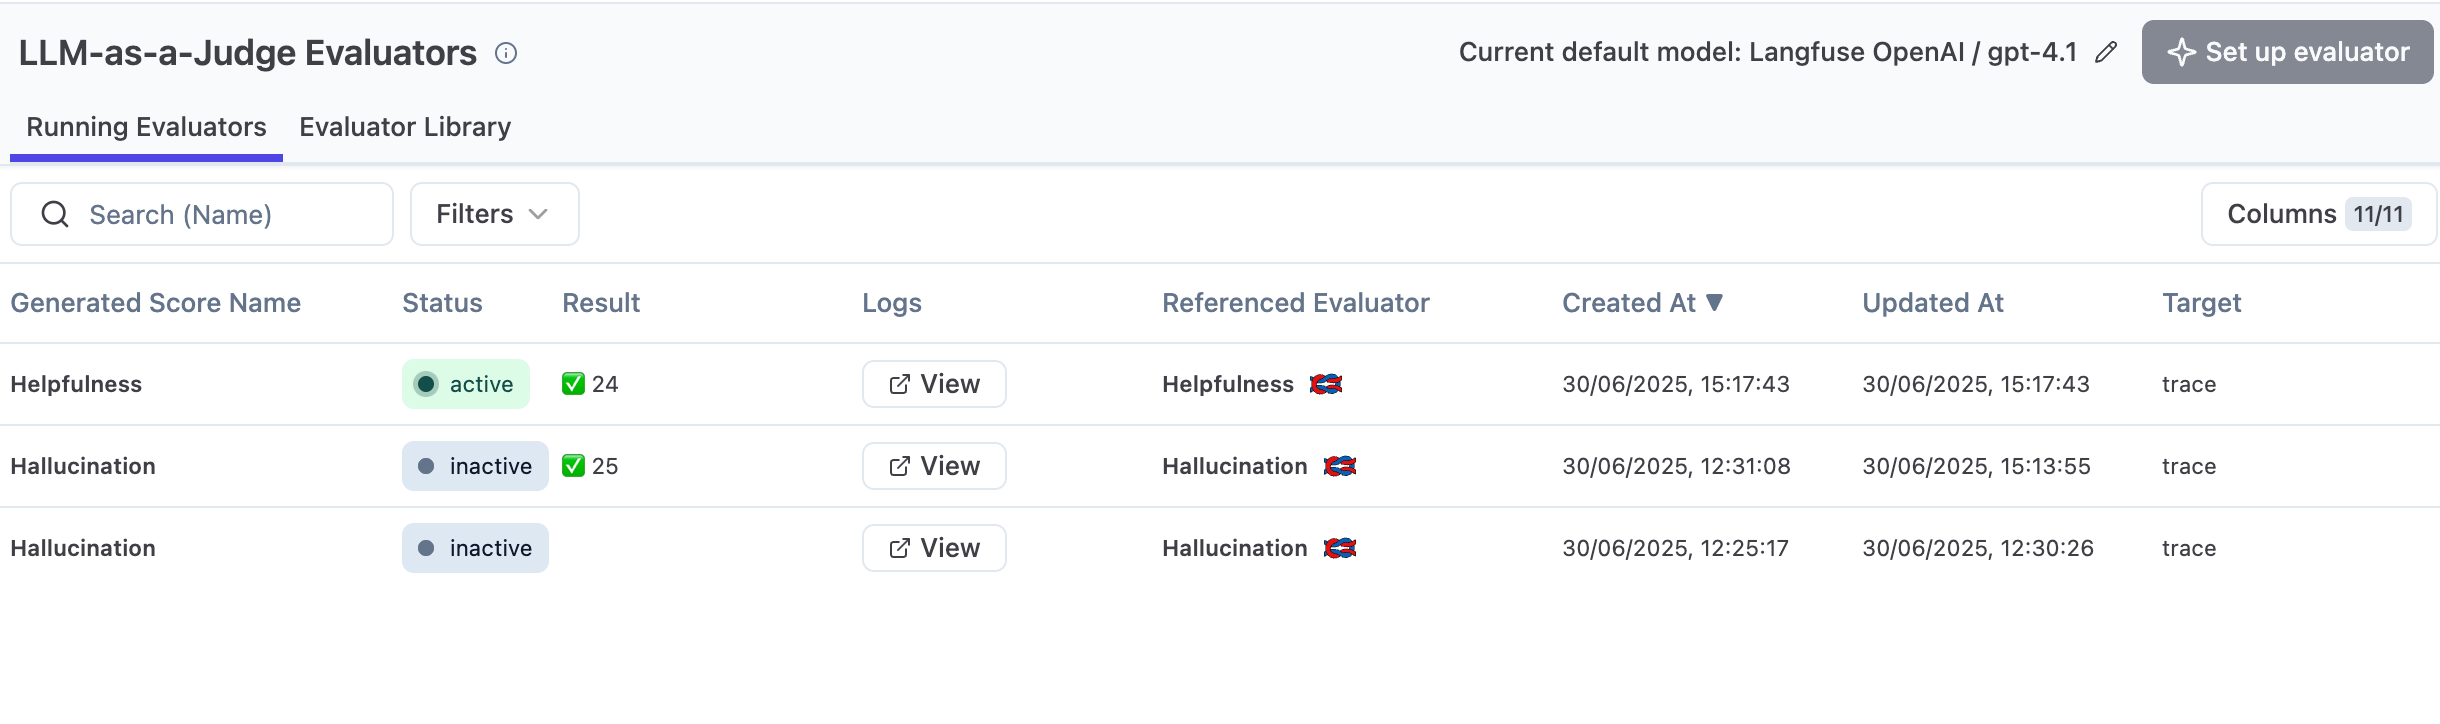
\includegraphics[width=0.8\linewidth,keepaspectratio]{aiagents54}
		
		{\tiny (Ref: Vizuara AI Agents Bootcamp Day 6)}
		\end{center}	
    % \end{column}
  % \end{columns}
\end{frame}

%%%%%%%%%%%%%%%%%%%%%%%%%%%%%%%%%%%%%%%%%%%%%%%%%%%%%%%%%%%
\begin{frame}[fragile]\frametitle{Quality Metrics for Agent Evaluation}

      \begin{itemize}
		\item \textbf{Hallucinations (Faithfulness):} Check if agent outputs information not grounded in sources
		\item \textbf{Trustworthiness:} Measure reliability and correctness of answers
		\item Integration with external evaluators like Cleanlab's Trustful LLM
		\item \textbf{Relevance:} Ensure outputs actually relevant to user's query
		\item \textbf{Correctness \& Completeness:} Verify all locations found and correctly matched
		\item Custom metrics for domain-specific checks supported
		\item Automated evaluation prompts check answers against retrieved context
	  \end{itemize}

\end{frame}

%%%%%%%%%%%%%%%%%%%%%%%%%%%%%%%%%%%%%%%%%%%%%%%%%%%%%%%%%%%
\begin{frame}[fragile]\frametitle{Browser Agents: AI with Internet Superpowers}
% \begin{columns}
    % \begin{column}[T]{0.6\linewidth}
      \begin{itemize}
		\item Specialized agents designed to interact with the web
		\item Can perform searches, click links, scrape and read webpages
		\item Extract information from online sources in real-time
		\item Serve as eyes and ears of AI in vast world of online data
		\item Bridge gap when LLM lacks factual data in internal knowledge
		\item Use tools like Google Search API and web page readers
		\item Essential for up-to-date information retrieval tasks
	  \end{itemize}
    % \end{column}
    % \begin{column}[T]{0.4\linewidth}
		\begin{center}
		
\includegraphics[width=0.6\linewidth,keepaspectratio]{aiagents55}
		
		{\tiny (Ref: Vizuara AI Agents Bootcamp Day 6)}
		\end{center}	
    % \end{column}
  % \end{columns}
\end{frame}

%%%%%%%%%%%%%%%%%%%%%%%%%%%%%%%%%%%%%%%%%%%%%%%%%%%%%%%%%%%
\begin{frame}[fragile]\frametitle{Key Takeaways: Multi-Agent Architecture Benefits}

      \begin{itemize}
		\item Multi-agent architectures open new possibilities and efficiencies
		\item Agent collaboration solves complex tasks more cleanly than solo agents
		\item Right tools distributed among expert agents yield better results
		\item Tracing and evaluation become safety net for autonomous agents
		\item Langfuse provides detailed execution tracing and evaluation dashboards
		\item Metrics like hallucination, trustworthiness, and relevance ensure quality
		\item Essential for building reliable, factual, and trustworthy AI systems
	  \end{itemize}

\end{frame}